\documentclass[../EDF Master Thesis.tex]{subfiles}

\begin{document}
    Ein Teil der Aufgabenstellung beinhaltet das Erstellen von zwei Demo Applikationen, welche die Funktion des \ac{edf} Schedulers unter Beweis stellen.

    \subsection{Blinky Demo} \label{section:blinky_demo}
        Für eine optische Vorführung des \ac{edf} Schedulers wurde eine 'Blinky Demo' erstellt, welche drei \ac{edf} Tasks beinhaltet.
        Jede der drei Tasks toggelt eine unterschiedliche \ac{led}, besitzen jedoch die gleichen \ac{edf} Parameter, welche in \autoref{table:blinky_demo_task_parameter} dargestellt sind.

        \begin{table}[ht!]
            \centering
            \begin{tabular}{l|c|c|c}
                Taskname & Periode & Deadline & \ac{wcet} \\
                \hline
                Task 1 & 50 & 100 & 100\\
                Task 2 & 50 & 100 & 100\\
                Task 3 & 50 & 100 & 100\\
            \end{tabular}
            \caption{Blinky Demo Task Parameter}
            \label{table:blinky_demo_task_parameter}
        \end{table}

        Die drei Tasks wurden exakt so gewählt, dass Sie die verschiedenen möglichen Status des \ac{edf} Schedulers simuliert und optisch dargestellt werden.
        Der Benutzer kann mit Hilfe des integrierten Button auf dem STM32F769I-Disc0 Board die drei Tasks, wie in \autoref{fig:blinky_demo_ablaufdiagramm} zu sehen, erstellen und löschen.
        
        \begin{figure}[H]
            \centering
            \resizebox{0.8\textwidth}{!}{%
                \begin{tikzpicture}[node distance = 2cm, auto]
                    % \draw[very thin,lightgray](-2,-9)grid[step=.5cm]+(6,10);
                
                    % Place nodes
                    \node [papProcess](pro1){Warten auf Benutzer};
                    \node [papProcess, below = of pro1](pro2){Idle Task};
                    \node [left = of pro2, xshift=-1cm](label21){Status 1};
                    \node [right = of pro2, xshift=-1cm](label22){\small\parbox{4cm}{Button Counter: 1 \\\ac{cpu}-Auslastung: 0\%}};
                    \node [papProcess, below = of pro2](pro3){Task 1 + Idle Task};
                    \node [left = of pro3, xshift=-1cm](label31){Status 2};
                    \node [right = of pro3, xshift=-1cm](label32){\small\parbox{4cm}{Button Counter: 2 \\\ac{cpu}-Auslastung: 50\%}};
                    \node [papProcess, below = of pro3](pro4){Task 1 + Task 2};
                    \node [left = of pro4, xshift=-1cm](label41){Status 3};
                    \node [right = of pro4, xshift=-1cm](label42){\small\parbox{4cm}{Button Counter: 3 \\\ac{cpu}-Auslastung: 100\%}};
                    \node [papProcess, below = of pro4](pro5){Task 1 + Task 2 + Task 3};
                    \node [left = of pro5, xshift=-1cm](label51){Status 4};
                    \node [right = of pro5, xshift=-1cm](label52){\small\parbox{4cm}{Button Counter: 4 \\\ac{cpu}-Auslastung: 150\%}};
                    \node [papProcess, below = of pro5](pro6){Task 2 + Task 3};
                    \node [left = of pro6, xshift=-1cm](label61){Status 5};
                    \node [right = of pro6, xshift=-1cm](label62){\small\parbox{4cm}{Button Counter: 5 \\\ac{cpu}-Auslastung: 100\%}};
                    \node [papProcess, below = of pro6](pro7){Task 3 + Idle Task};
                    \node [left = of pro7, xshift=-1cm](label77){Status 6};
                    \node [right = of pro7, xshift=-1cm](label72){\small\parbox{4cm}{Button Counter: 6 \\\ac{cpu}-Auslastung: 50\%}};
                    % invisible node helpful later
                    \node[left=1cm of pro6,scale=0.05](inv){};
                
                    % Draw edges
                    \path [line] (pro1) -- (pro2);
                    \path [line] (pro2) -- (pro3);
                    \path [line] (pro3) -- (pro4);
                    \path [line] (pro4) -- (pro5);
                    \path [line] (pro5) -- (pro6);
                    \path [line] (pro6) -- (pro7);
                    \path[-,draw] (pro7) -| node{} (inv.north);
                    \path[line]{} (inv.north) |- node[above]{reset} (pro2);
                \end{tikzpicture}  
            }%
            \caption{Blinky Demo Ablaufdiagramm}
            \label{fig:blinky_demo_ablaufdiagramm}
        \end{figure} 
        
        Die Eigenschaften der einzelnen Status aus \autoref{fig:blinky_demo_ablaufdiagramm} sind wie folgt:
        \begin{itemize}
            \item \textbf{Warten auf Benutzer}: Anfangs ist keine \ac{edf} Task gestartet, die \ac{led}s leuchten dauerhaft und die Idle Task wird dauerhaft ausgeführt.
            \item \textbf{Status 1}: Sobald der Benutzer zum ersten Mal den Button drückt, wird 'Task 1' erstellt und ausgeführt.
                Nun blinkt die erste \ac{led} regelmäßig, die anderen beiden \ac{led}s leuchten noch dauerhaft.
                Durch diese Konstellation teilen sich 'Task 1' und die Idle Task die \ac{cpu}-Zeit und es ergibt sich eine \ac{cpu}-Auslastung von 50\%.
            \item \textbf{Status 2}: Wird nun der Button ein zweites Mal gedrückt, wird 'Task 2' erstellt und es blinkt nun auch die zweite \ac{led} regelmäßig.
                Aufgrund der Taskparameter von 'Task 1' und 'Task 2' teilen sich die beiden Tasks die komplette \ac{cpu}-Zeit und lasten diese zu 100\% aus, dadurch wird die Idle Task nicht mehr ausgeführt.
            \item \textbf{Status 3}: Drückt der Benutzer nun ein drittes Mal den Button, wird 'Task 3' erstellt, die dritte \ac{led} fängt nun auch an zu blinken.
                Aufgrund der gewählten Taskparameter beträgt die \ac{cpu}-Auslastung nun 150\%, hier kann der \ac{edf} Scheduler die einzelnen Deadlines nicht einhalten.
                Dies wird anhand der \ac{led}s sichtbar, da diese nun nur noch unregelmäßig blinken.
                Des Weiteren, sofern der Debug Mode aktiviert ist, können die nicht eingehaltenen Deadlines der Tasks über die \ac{usart} Schnittstelle, sowie welche Task wie oft ihre Deadline verfehlt hat, ausgelesen werden.
            \item \textbf{Status 4}: Wird nun der Button ein weiteres Mal gedrückt, wird 'Task 1' gelöscht und die erste \ac{led} wird ausgeschaltet.
                Nun teilen sich 'Task 2' und 'Task 3' die \ac{cpu}-Zeit und die \ac{cpu}-Auslastung beträgt noch 100\%, aus diesem Grund wird die Idle Task auch nicht aufgerufen.
            \item \textbf{Status 5}: Ein weiteres Drücken des Buttons löscht 'Task 2' und 'Task 3' teilt sich mit der Idle Task jeweils die hälfte der \ac{cpu}-Zeit.
            \item \textbf{Status 6}: Drückt der Benutzer nun ein weiteres Mal den Button wird 'Task 3' gelöscht und alle drei \ac{led}s leuchten dauerhaft.
                Die \ac{cpu}-Auslastung liegt nun bei 0\%, dadurch wird die Idle Task dauerhaft ausgeführt.
                Das System befindet sich nun wieder am Anfang der Ausführung und kann erneut die einzelnen Status ausführen.
        \end{itemize}

    \subsection{\ac{fft} Demo} \label{section:fft_demo}

        Für die zweite Applikation erstellt und sendet ein Host-Computer ein Signal, bestehend aus einem oder mehreren Sinus- oder Kosinus-Signalen, an den Mikrocontroller über das \ac{udp} Protokoll gesendet wird.
        Der Mikrocontroller führt, basierend auf dem empfangenen Signal, eine \ac{fft}-Berechnung aus und sendet die Ergebnisse an den Host-Computer zurück.
        Für das Erstellen und Senden eines Signals, der Empfang der Ergebnisse und das darstellen der Signale wurde eine \ac{gui}, basierend auf der Programmiersprache Python erstellt.
        Des Weiteren wurden für die Kommunikation mit dem Host-Computer, sowie die Berechnung der \ac{fft} drei \ac{edf} Tasks erstellt, welche folgende Eigenschaften besitzen:

        \begin{table}[ht!]
            \centering
            \begin{tabular}{l|c|c|c|l}
                Taskname & Periode & Deadline & \ac{wcet} & Aufgabe \\
                \hline
                Task 1 & 10 & 10 & 2 & Empfangen des Signals über \ac{udp}\\
                Task 2 & 10 & 10 & 2 & Berechnung der \ac{fft}\\
                Task 3 & 10 & 10 & 2 & Senden der \ac{fft} Ergebnisse über \ac{udp}
            \end{tabular}
            \caption{Blinky Demo Task Parameter}
            \label{table:blinky_demo_task_parameter}
        \end{table}

        Der komplette Ablauf der einzelnen Komponenten sieht wie folgt aus:

        \begin{figure}[H]
            \centering
            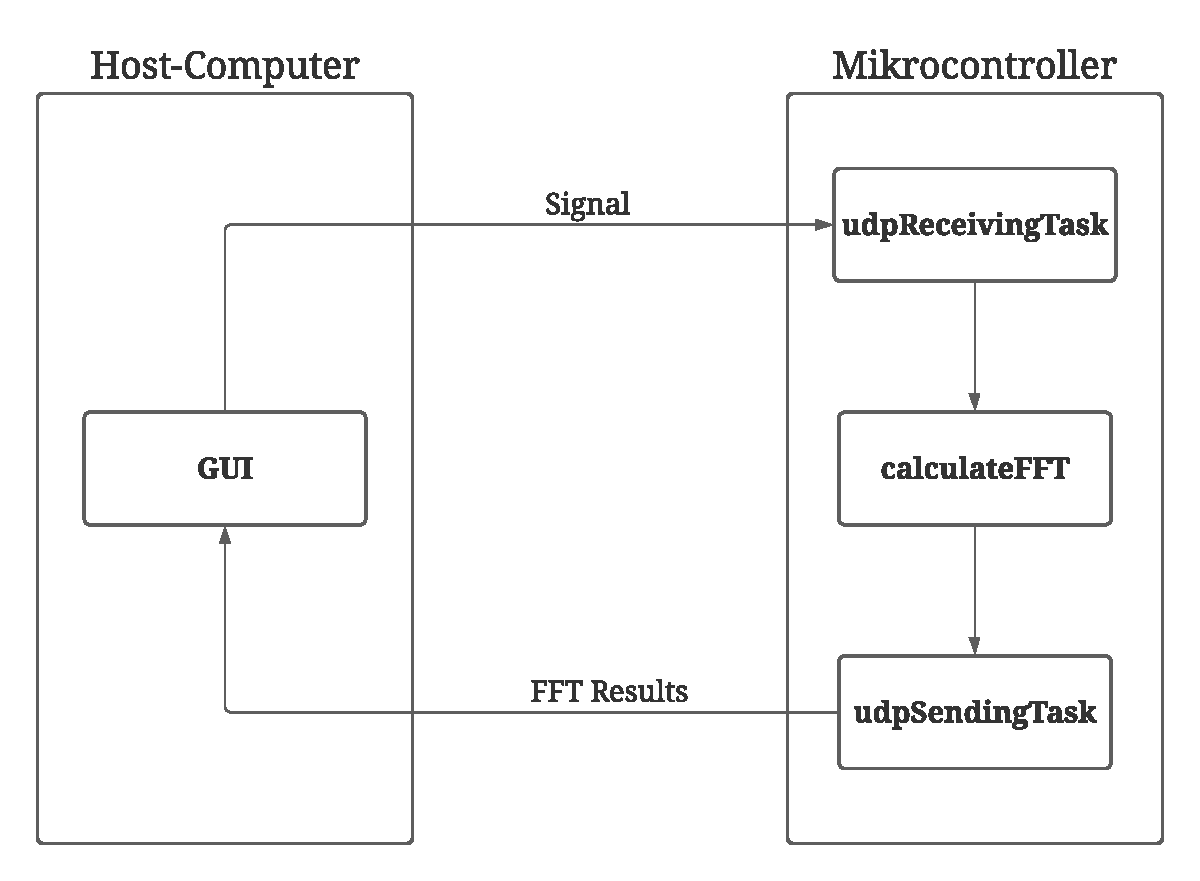
\includegraphics[height=10cm, width=14cm]{./attachments/FFT Ablauf.pdf}
            \caption{\ac{fft} Demo Ablaufdiagramm}
            \label{fig:fft_demo_ablaufdiagramm}
        \end{figure}

        \clearpage
        \subsubsection{\ac{gui}}
            Die \ac{gui} wurde für eine einfache Bedienung und einer übersichtlichen Anzeige gestaltet und ist in \autoref{fig:gui} abgebildet:

            \begin{figure}[H]
                \centering
                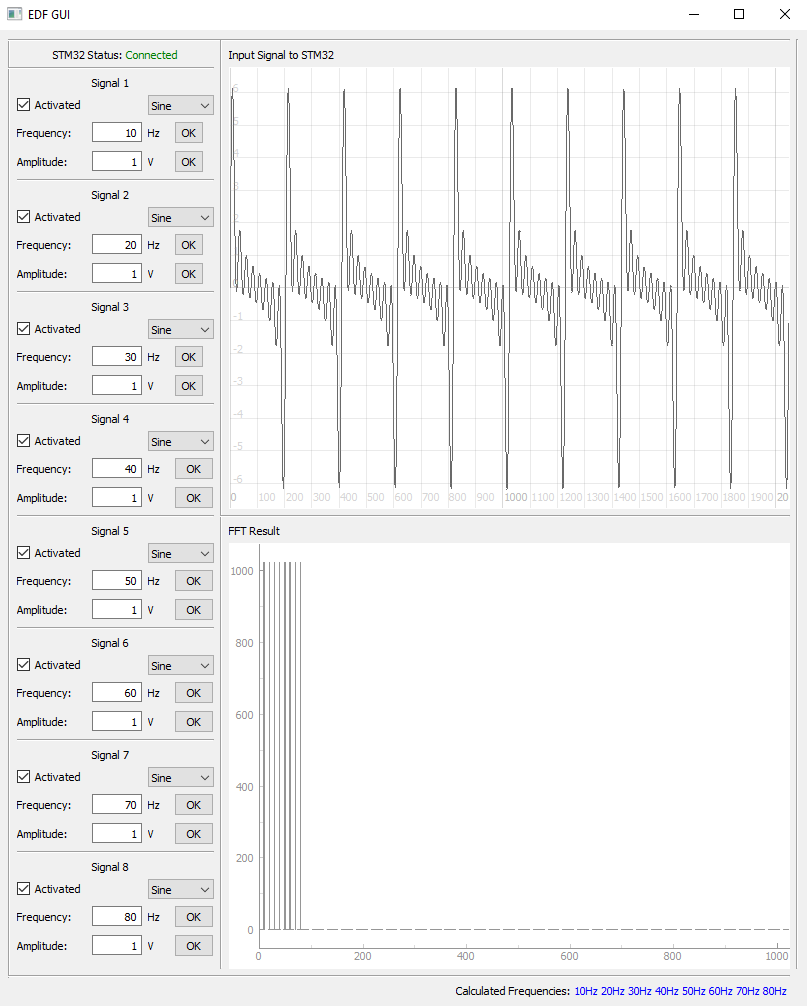
\includegraphics[width=0.97\textwidth]{./attachments/gui.png}
                \caption{\ac{gui} Interface}
                \label{fig:gui}
            \end{figure}

        In der linken oberen Ecke wird der Verbindungsstatus zum Mikrocontroller angezeigt, darunter kann der Benutzer bis zu acht Signale aktiveren oder deaktivieren, sowie auch deren Eigenschaften verändern.
        Das resultierende Signal wird dann zentral in dem oberen Plotfenster dargestellt.
        Im unteren Plot werden die Ergebnisse der \ac{fft}-Berechnung angezeigt, zusätzlich werden die erkannten Frequenzen in Textform angezeigt.

        \subsubsection{Tasks des Mikrocontrollers}

\end{document}